\documentclass{article}
\usepackage{tikz}
\usepackage{hyperref}
\usepackage{mhchem}
\usepackage[a4paper]{geometry}
\usepackage{fancyhdr}
\pagestyle{fancy}
\lhead{Fotosynthese}
\rhead{Januar 2026}
\begin{document} 
Die \emph{Fotosynthese} beschreibt den Prozess der Glucosegewinnung von Pflanzen. Dabei Reagiert, unter Energiezufuhr durch Sonnenlicht, Wasser und Kohlenstoffdioxid zu Sauerstoff und Glucose.
\[
 \ce{6H2O + 6CO2 ->[Licht] 6O2 + C6H12O6} 
\] 
 
\subsection{Ablauf}
Die Fotosynthese kann in zwei hauptsächliche Reaktionen aufgeteilt werden, die \hyperref[Die Primärreaktion]{Primärreaktion} und die \hyperref[Die Sekundärreaktion]{Sekundärreaktion}. 
 
Hier stehen \ce{NADP+ + ADP + P <-> NADPH+H+ + ATP} in einer art Zyklus.

Die Primärreaktion verarbeitet mithilfe von Lichtenergie Wasser zu Sauerstoff, wobei sie chemische Energie in Form von \ce{ATP} und \ce{NADPH + H+} produziert. Diese können dann von der Sekundärreaktion genutzt werden um \ce{C6H12O6} aus \ce{CO2} zu produzieren.
\begin{center} 
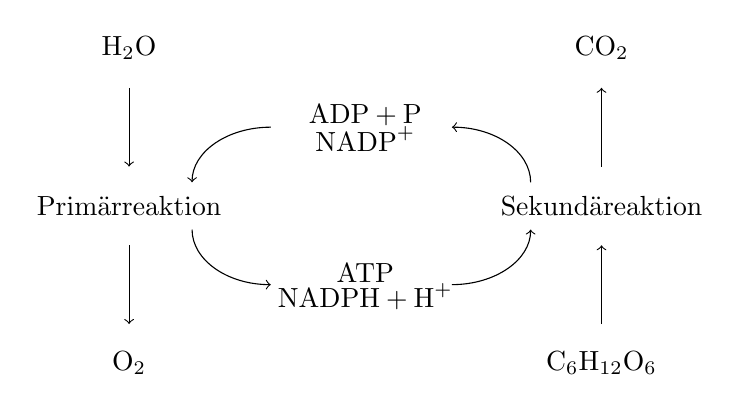
\begin{tikzpicture}
 \draw (0, 0) node{\ce{H2O}};
 \draw[->] (0, -0.5) -- (0, -1.5); 
 \draw (0, -2) node{Primärreaktion};
 \draw[->] (0, -2.5) -- (0, -3.5); 
 \draw (0, -4) node{\ce{O2}}; 

 \draw (6, 0) node{\ce{CO2}};
 \draw[->] (6, -1.5) -- (6, -0.5); 
 \draw (6, -2) node{Sekundäreaktion};
 \draw[->] (6, -3.5) -- (6, -2.5); 
 \draw (6, -4) node{\ce{C6H12O6}}; 
 
 \draw (3, -0.85) node{\ce{ADP + P}}; 
 \draw (3, -1.15) node{\ce{NADP+}}; 
 
 \draw (3, -2.85) node{\ce{ATP}}; 
 \draw (3, -3.15) node{\ce{NADPH + H+}};
 
 \draw[->] (1.8,-1) arc (90:180:1 and 0.7);
 \draw[->] (0.8,-2.3) arc (180:270:1 and 0.7);
 \draw[->] (4.1,-3) arc (270:360:1 and 0.7);
 \draw[->] (5.1,-1.7) arc (0:90:1 and 0.7);
\end{tikzpicture} 
\end{center} 
\end{document}